\documentclass[11pt,letterpaper]{article}
\usepackage[left=1.25in,right=1.25in,top=1in,bottom=1in]{geometry}
\usepackage{fontspec}
\setmainfont{texgyretermes}[Extension=.otf,UprightFont=*-regular,BoldFont=*-bold,ItalicFont=*-italic,BoldItalicFont=*-bolditalic]
\setsansfont{texgyreheros}[Extension=.otf,UprightFont=*-regular,BoldFont=*-bold,ItalicFont=*-italic,BoldItalicFont=*-bolditalic]
\usepackage{amsmath,amssymb,graphicx,booktabs,longtable,tabularx,array}
\usepackage{setspace,microtype,xcolor,titlesec,enumitem,caption,float,placeins,needspace}
\usepackage{tikz}
\usetikzlibrary{arrows.meta,positioning,fit,calc}
\usepackage[authoryear,round]{natbib}
\usepackage{xurl}
\usepackage{fancyhdr}
\usepackage[unicode,colorlinks=true,linkcolor=headingblue,citecolor=headingblue,urlcolor=headingblue]{hyperref}
\definecolor{headingblue}{HTML}{365F91}
\definecolor{softblue}{HTML}{EEF3FB}
\definecolor{softgreen}{HTML}{EFF6F0}
\definecolor{softpurple}{HTML}{F3EFF8}
\setstretch{1.15}
\setlength{\parindent}{0pt}
\setlength{\parskip}{7pt}
\setlength{\emergencystretch}{2em}
\setlength{\tabcolsep}{5pt}
\renewcommand{\arraystretch}{1.18}
\titleformat{\section}{\color{headingblue}\bfseries\fontsize{14}{17}\selectfont}{\thesection}{.6em}{}
\titleformat{\subsection}{\color{headingblue}\bfseries\fontsize{12}{15}\selectfont}{\thesubsection}{.6em}{}
\titleformat{\subsubsection}{\bfseries\fontsize{11}{14}\selectfont}{\thesubsubsection}{.6em}{}
\titlespacing*{\section}{0pt}{18pt}{8pt}
\titlespacing*{\subsection}{0pt}{12pt}{5pt}
\setlist{nosep,leftmargin=1.5em,topsep=4pt}
\captionsetup{font=small,labelfont=bf,skip=6pt}
\pagestyle{fancy}
\fancyhf{}
\fancyhead[L]{\small\color{gray}StereoDetect}
\fancyhead[R]{\small\color{gray}IOE-414: Deep Learning}
\fancyfoot[C]{\thepage}
\fancypagestyle{plain}{\fancyhf{}\fancyhead[L]{\small\color{gray}StereoDetect}\fancyhead[R]{\small\color{gray}IOE-414: Deep Learning}\fancyfoot[C]{\thepage}\renewcommand{\headrulewidth}{.3pt}}
\renewcommand{\headrulewidth}{.3pt}
\setlength{\headheight}{14pt}
\renewcommand{\contentsname}{Table of Contents}
\setcounter{tocdepth}{2}
\newcommand{\reportsection}[1]{\clearpage\section{#1}}
\newcommand{\code}[1]{{\small\nolinkurl{#1}}}
\makeatletter
\let\tableinput\@@input
\makeatother
\newcommand{\pct}[1]{#1\%}
% Editable cover and submission details.
\newcommand{\ProjectTitle}{StereoDetect: Explainable Stereotype Detection with Encoder Models and Qwen3.5-2B}
\newcommand{\MemberOne}{Mugupuram Kavya Amrutha}
\newcommand{\RegisterOne}{2023BCS0221}
\newcommand{\MemberTwo}{Harissh Ragav Dhamodaran}
\newcommand{\RegisterTwo}{2023BCD0059}
\newcommand{\SubmissionMonth}{October--2026}
\newcommand{\ProjectGithub}{\url{https://github.com/GL3MON/explainable-stereotype-detection}}

\hypersetup{pdftitle={StereoDetect: Explainable Stereotype Detection},pdfauthor={Harissh Ragav Dhamodaran and Mugupuram Kavya Amrutha},pdfsubject={Deep Learning Minor Project Report}}

\begin{document}
\hypersetup{pageanchor=false}
\begin{titlepage}
\centering
{\fontsize{16}{20}\selectfont\bfseries INDIAN INSTITUTE OF\par INFORMATION TECHNOLOGY KOTTAYAM\par}
\vspace{.18in}
{\fontsize{12}{15}\selectfont (An Institute of National Importance)\par}
\vspace{.3in}

\includegraphics[width=1.65in]{figures/institute_logo.jpeg}\par
\vspace{.3in}
{\fontsize{14}{18}\selectfont\bfseries IOE-414: DEEP LEARNING\par}
\vspace{.16in}
{\fontsize{14}{18}\selectfont\bfseries MINOR PROJECT REPORT\par}
\vspace{.35in}
{\fontsize{14}{18}\selectfont\textbf{Project Title:}\par}
\vspace{.12in}
{\fontsize{17}{21}\selectfont\bfseries\ProjectTitle\par}
\vspace{.4in}
{\fontsize{14}{18}\selectfont\textbf{Group Members:}\par}
\vspace{.13in}
\begin{tabular}{ll}
\MemberOne & \RegisterOne\\[7pt]
\MemberTwo & \RegisterTwo
\end{tabular}\par
\vfill
{\fontsize{12}{16}\selectfont Department of Computer Science and Engineering\par}
\vspace{.18in}
{\fontsize{12}{16}\selectfont\SubmissionMonth\par}
\end{titlepage}

\hypersetup{pageanchor=true}
\pagenumbering{roman}
\begingroup
\setstretch{1.0}\setlength{\parskip}{0pt}\small
\tableofcontents
\endgroup
\clearpage
\section*{Abstract}
\addcontentsline{toc}{section}{Abstract}
Stereotype detection requires a classifier to distinguish group generalizations from counter-stereotypical descriptions, neutral statements, and bias. This project develops a reproducible five-class classification and explanation pipeline on the local StereoDetect benchmark splits. It compares ALBERT and ModernBERT encoders with Qwen3.5-2B under three explicitly separated tasks: (A) sentence to label, (B) sentence to category, target, and label in JSON, and (C) sentence plus supplied category and target to label. Each Qwen task is evaluated using the pretrained checkpoint and a separate supervised fine-tuned (SFT) LoRA adapter, with thinking disabled.

The experiments use 6,080 training, 868 validation, and 1,738 test examples. Task A improves from 23.19\% to 93.84\% label accuracy and from 14.21\% to 93.89\% macro F1 after SFT. Task B achieves 93.61\% label accuracy, 99.37\% category accuracy, 98.16\% exact target accuracy, and 92.87\% accuracy when all three fields must match together. Task C achieves 95.51\% label accuracy with gold category and target annotations supplied as input. The saved ModernBERT-large run reaches 93.33\% accuracy and 93.39\% macro F1, while ALBERT reaches 88.09\% and 88.20\%, respectively.

Word-level LIME and Kernel SHAP explanations are examined using two saved ModernBERT-large examples, including a misclassification, with signed color maps and legends. Error analysis identifies the stereotype/anti-stereotype boundary as a major remaining difficulty. The report presents prediction metrics and word-level sensitivity analyses for the evaluated models, with explicit task inputs and output-scoring rules.

\textbf{Keywords:} stereotype detection; StereoDetect; Qwen3.5; LoRA; ModernBERT; ALBERT; LIME; SHAP.

\subsection*{Base Paper Details}
\addcontentsline{toc}{subsection}{Base Paper Details}
\textbf{Primary benchmark paper.}
\begin{description}[style=nextline,leftmargin=0pt]
\item[Title:] StereoDetect: Detecting Stereotypes and Anti-stereotypes the Correct Way Using Social Psychological Underpinnings.
\item[DOI:] \url{https://doi.org/10.18653/v1/2025.findings-emnlp.216}
\item[Conference / publication:] \textit{Findings of the Association for Computational Linguistics: EMNLP 2025}, pp.\ 4051--4082.
\item[Authors:] Kaustubh Shivshankar Shejole and Pushpak Bhattacharyya.
\item[Year:] 2025.
\end{description}
\Needspace{4\baselineskip}
The benchmark paper provides the conceptual and dataset basis for the five-class task \citep{shejole2025}. This project uses its local sentence-classification CSV splits and implements additional encoder, SFT, and explanation workflows.

\textbf{Complementary methodology paper.}
\begin{description}[style=nextline,leftmargin=0pt]
\item[Title:] HEARTS: A Holistic Framework for Explainable, Sustainable and Robust Text Stereotype Detection.
\item[DOI:] \url{https://doi.org/10.18653/v1/2025.ijcnlp-long.1}
\item[Conference / publication:] \textit{Proceedings of the 14th International Joint Conference on Natural Language Processing and the 4th Conference of the Asia-Pacific Chapter of the Association for Computational Linguistics}, pp.\ 1--18.
\item[Authors:] Theo King, Zekun Wu, Adriano Koshiyama, Emre Kazim, and Philip Colin Treleaven.
\item[Year:] 2025.
\end{description}
HEARTS motivates the lightweight ALBERT baseline and paired LIME/SHAP analysis \citep{king2025}. Our five-label StereoDetect experiments differ from its binary EMGSD setup; the project is an adaptation rather than an exact reproduction of its dataset or reported scores.

\clearpage
\pagenumbering{arabic}
\reportsection{Problem Statement}
\subsection{Motivation and task definition}
A statement about a social group can express a conventional association, contradict such an association, describe an individual neutrally, or convey bias. Recognizing a target word alone does not resolve these distinctions. The same vocabulary can occur in both stereotypical and anti-stereotypical descriptions, while a seemingly favorable group generalization can still be a stereotype. A useful system must therefore classify the sentence in context and make its decision available for inspection.

StereoDetect separates stereotype and anti-stereotype detection from a broader measurement of model bias \citep{shejole2025}. Following the label mapping supplied with the local data, this project assigns each sentence one of five labels: anti-stereotype (0), stereotype (1), neutral without target term (2), neutral with target term (3), or bias (4). The class names describe dataset annotations. They should not be interpreted as a universal, context-free judgment about every possible utterance.

Let $s$ denote a sentence, $c$ its category, $t$ its target-group string, and $y\in\{0,1,2,3,4\}$ its label. The project studies three Qwen input/output contracts:
\begin{align}
\text{Task A:}\quad & f_A(s)\longrightarrow y,\\
\text{Task B:}\quad & f_B(s)\longrightarrow (c,t,y),\\
\text{Task C:}\quad & f_C(s,c,t)\longrightarrow y.
\end{align}
Task B returns one JSON object containing all three predicted fields. Task C receives \emph{gold} category and target annotations from the dataset, referred to as \emph{auxiliary annotations}. Its score answers a conditional classification question and should be interpreted separately from the sentence-only tasks.

\subsection{Project objectives}
\begin{enumerate}
\item Establish sentence-only encoder baselines using ALBERT and ModernBERT on the supplied train, validation, and test splits.
\item Evaluate Qwen3.5-2B in all three tasks, comparing the base checkpoint with a task-specific SFT adapter for each task.
\item Report label accuracy and macro F1 consistently, with category, target, and complete-record accuracy added for JSON generation.
\item Analyze class-level errors and inspect selected encoder decisions using aligned word-level LIME and Kernel SHAP explanations.
\end{enumerate}

\subsection{Scope and contribution}
The work combines supervised classification, parameter-efficient adaptation, structured prediction, and post-hoc explanations in one local implementation. The main experimental contribution is the comparison of three clearly specified Qwen tasks under both base and SFT states. A separate adapter is trained for each task; the three SFT results are not three inference modes of a single jointly trained adapter.

The encoder workflows consume only the sentence. The explanation component operates on saved encoder classifiers and reuses their class probabilities under masked-word perturbations. The report's word color maps explain ModernBERT-large decisions. The model comparison also includes the MiniLM and Qwen3-Embedding baseline scores recorded in the review document.

\reportsection{Method Overview with Architecture}
\subsection{End-to-end pipeline}
The implementation separates data loading, model training, evaluation, prediction, and explanation into explicit workflows. The benchmark dataset is loaded and converted into inputs appropriate for the selected task. Training uses only the training split; validation macro F1 determines checkpoint selection. The selected model or adapter is then evaluated on the complete test split. Saved predictions support independent recomputation of the report tables.

\begin{figure}[H]
\centering
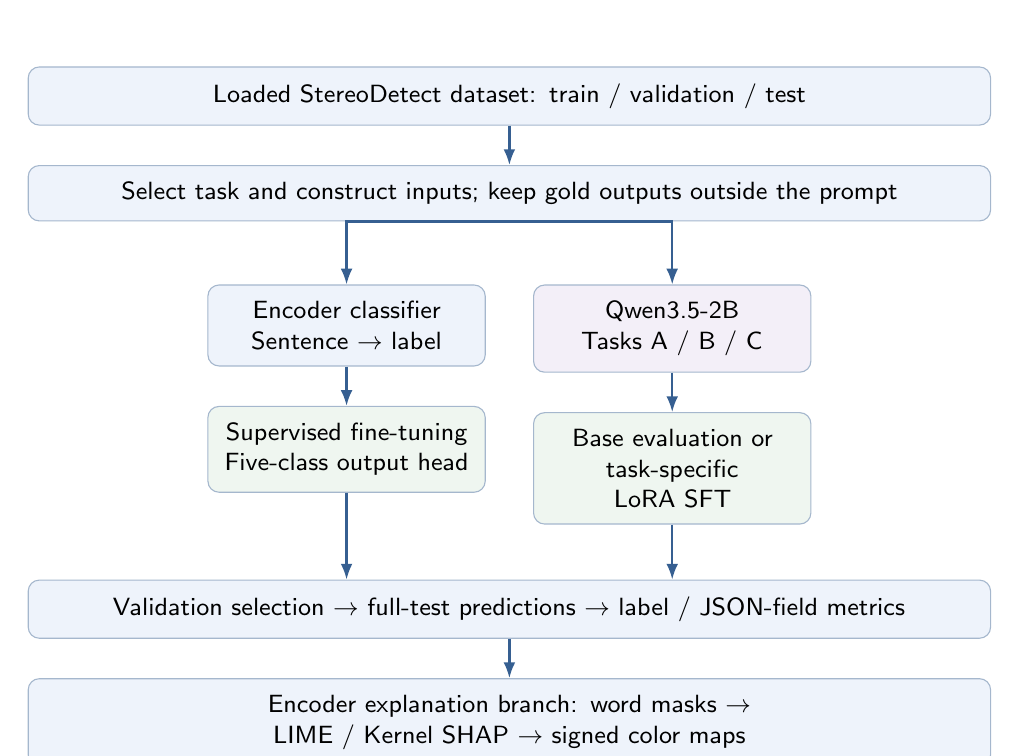
\begin{tikzpicture}[node distance=5mm and 6mm, font=\sffamily\small,
block/.style={draw=headingblue!45,rounded corners,fill=softblue,align=center,inner sep=6pt,text width=3.1cm},
wide/.style={block,text width=11.8cm},arr/.style={-{Latex[length=2mm]},thick,draw=headingblue}]
\node[wide] (data) {Loaded StereoDetect dataset: train / validation / test};
\node[wide,below=of data] (contract) {Select task and construct inputs; keep gold outputs outside the prompt};
\node[block,below left=8mm and 3mm of contract.south] (enc) {Encoder classifier\\Sentence $\to$ label};
\node[block,below right=8mm and 3mm of contract.south,fill=softpurple] (qwen) {Qwen3.5-2B\\Tasks A / B / C};
\node[block,below=of enc,fill=softgreen] (trainenc) {Supervised fine-tuning\\Five-class output head};
\node[block,below=of qwen,fill=softgreen] (trainqwen) {Base evaluation or\\task-specific LoRA SFT};
\node[wide,below=9mm of $(trainenc.south)!0.5!(trainqwen.south)$] (eval) {Validation selection $\to$ full-test predictions $\to$ label / JSON-field metrics};
\node[wide,below=of eval] (explain) {Encoder explanation branch: word masks $\to$ LIME / Kernel SHAP $\to$ signed color maps};
\draw[arr] (data)--(contract);
\draw[arr] (contract.south)-|(enc.north);\draw[arr] (contract.south)-|(qwen.north);
\draw[arr] (enc)--(trainenc);\draw[arr] (qwen)--(trainqwen);
\draw[arr] (trainenc.south)--(trainenc.south |- eval.north);
\draw[arr] (trainqwen.south)--(trainqwen.south |- eval.north);
\draw[arr] (eval)--(explain);
\end{tikzpicture}
\caption{Implemented pipeline. The last branch explains encoder outputs. It is not a Qwen reasoning-generation stage.}
\label{fig:pipeline}
\end{figure}

\subsection{Encoder and embedding model families}
\textbf{ALBERT.} ALBERT reduces parameter requirements through factorized embeddings and cross-layer parameter sharing \citep{lan2020}. The project loads \code{albert/albert-base-v2} using a sequence-classification model with five outputs. Tokenized sentence inputs pass through the encoder and its classification head to produce logits, followed by a softmax for class probabilities. Category and target remain in the saved rows for analysis and are excluded from encoder input.

\textbf{ModernBERT.} ModernBERT modernizes the bidirectional encoder architecture, including rotary positional information and alternating attention patterns \citep{warner2024}. The saved project runs use \code{answerdotai/ModernBERT-base} and \code{answerdotai/ModernBERT-large} with five-class sequence-classification heads. The local sequence limit is 128 tokens, irrespective of the backbone's longer supported context. The same sentence-only contract enables a meaningful task-level comparison with ALBERT and Qwen task A, although hyperparameters and computational settings differ.

\textbf{Embedding baselines.} MiniLM supplies compact transformer representations through distillation \citep{wang2020}; Qwen3-Embedding provides decoder-derived embedding models \citep{zhang2025}. The five-class comparison includes scores for \code{all-MiniLM-L6-v2} and \code{Qwen3-Embedding-0.6B}. Qwen3-Embedding-0.6B is a different model family from the Qwen3.5-2B generative checkpoint used in tasks A--C.

\subsection{Qwen tasks and supervised adaptation}
The backbone is \code{Qwen/Qwen3.5-2B} \citep{qwen2026}. Here, \emph{base} means that this published checkpoint is evaluated without one of our StereoDetect task adapters. It does not imply that the checkpoint lacks any upstream instruction training. Text inputs use the language-model path; images are not part of the project dataset.

\begin{table}[H]
\centering\small
\caption{Three Qwen tasks, each evaluated in Base and SFT states.}
\label{tab:contracts}
\begin{tabularx}{\linewidth}{lXX}
\toprule Task & Input & Predicted output\\\midrule
A & Sentence & One integer label, 0--4\\
B & Sentence & JSON: category, target, and label\\
C & Sentence + gold category + gold target & One integer label, 0--4\\\bottomrule
\end{tabularx}
\end{table}

All three tasks explicitly disable thinking. Tasks A and C request a single digit without an explanation. At evaluation, the predicted label is selected by the largest next-token logit among the five numeric label tokens:
\begin{equation}
\hat y=\arg\max_{k\in\{0,1,2,3,4\}}\ell_k(s),
\end{equation}
with the category and target added to the prompt for task C. Normalizing these five logits produces a distribution over the five label choices.

Task B uses greedy, unconstrained generation of a JSON object with a saved maximum of 96 new tokens. Categories are normalized by trimming, case folding, and collapsing whitespace. Targets preserve dataset spelling, capitalization, and underscores. The label must be an integer in the permitted range. The training objective supervises the generated JSON fields, while checkpoint selection uses validation \emph{label} macro F1. This selection criterion does not directly optimize complete-record exact match.

LoRA freezes the backbone weights and adds trainable low-rank updates to selected language-model projections \citep{hu2022}. For a frozen matrix $W_0$, the adapted transformation can be written as
\begin{equation}
W=W_0+\frac{\alpha}{r}BA,
\end{equation}
where $A$ and $B$ are trainable low-rank matrices. The project uses rank $r=16$, scaling $\alpha=32$, and dropout 0.05. Attention, gated linear-attention, and feed-forward projection modules are targeted by the saved Qwen training implementation. Prompt tokens are masked from the causal training loss; assistant output tokens and their ending token contribute to supervision. Each task has its own adapter and prompt contract.

\subsection{Training protocol and checkpoint selection}
Table~\ref{tab:training} summarizes the saved settings. The ALBERT configuration adapts the six-epoch, effective-batch-64, learning-rate-$2\times10^{-5}$ setup recorded in the HEARTS reproduction notes to this five-label benchmark. ModernBERT-base includes an initial run and a separately retuned run. Multiple hyperparameters change in the retuned setup, so its improvement is not attributable to the learning rate alone.

\begin{table}[H]
\centering\scriptsize
\caption{Saved supervised training configurations. Batch is the global effective batch.}
\label{tab:training}
\begin{tabularx}{\linewidth}{Xrrrrl}
\toprule Run & Epochs & Batch & LR & Seed & Precision\\\midrule
ALBERT-base-v2 & 6 & 64 & $2\times10^{-5}$ & 42 & BF16 autocast\\
ModernBERT-base, original & 6 & 64 & $2\times10^{-5}$ & 42 & BF16 autocast\\
ModernBERT-base, retuned & 3 & 32 & $5\times10^{-5}$ & 3407 & BF16 autocast\\
ModernBERT-large & 3 & 32 & $3\times10^{-5}$ & 3407 & BF16 autocast\\
Qwen A: sentence-only SFT & 3 & 32 & $2\times10^{-4}$ & 42 & FP32\\
Qwen B: JSON SFT & 3 & 16 & $2\times10^{-4}$ & 42 & BF16\\
Qwen C: conditioned SFT & 3 & 16 & $2\times10^{-4}$ & 42 & BF16\\\bottomrule
\end{tabularx}
\end{table}

The completed sentence-only Qwen SFT job runs with DistributedDataParallel/NCCL on two Tesla T4 GPUs, using 16 examples per device, no gradient accumulation, and a global batch of 32. Its 6,080 training examples give 190 optimizer steps per epoch and 570 steps across three epochs. The saved run uses FP32, a cosine learning-rate schedule, a 5\% warmup fraction, AdamW, and 16,819,200 trainable adapter parameters. Epoch 3 is selected by validation macro F1. Training plus evaluation takes approximately 69.3 minutes in that job; this is a run-specific elapsed time, not a controlled throughput benchmark.

The local encoder runs use BF16 autocast and FP32 parameters. ModernBERT-large uses weight decay 0.01 and 30 warmup optimizer steps. The other Qwen SFT runs use micro-batch 4 and gradient accumulation 4. The base Qwen benchmarks run through vLLM in BF16, while the completed task-A adapter evaluation uses FP32 PyTorch. Consequently, the base/SFT differences are observed task-adaptation comparisons with different numerical runtimes, rather than isolated same-engine ablations.

\subsection{Aligned LIME and Kernel SHAP explanations}
LIME fits a local surrogate around a prediction by observing perturbed inputs \citep{ribeiro2016}. SHAP assigns additive feature contributions relative to a background input \citep{lundberg2017}. The implementation gives both methods the same word-occurrence feature space, preserving punctuation and position. Repeated occurrences of a word are separate features, using \code{bow=False}. Removing a feature replaces the associated word occurrence with the model's mask token.

The saved diagnostic configuration uses 1,000 LIME perturbations and up to 512 Kernel SHAP coalitions, with no L1 feature selection. Kernel SHAP uses an all-masked background and an identity link on classifier probabilities. Short examples can enumerate coalitions rather than consume the full sampling budget. For class $k$, the additive interpretation is
\begin{equation}
f_k(s)\approx E[f_k(s_{\mathrm{masked}})]+\sum_{j=1}^{m}\phi_{j,k},
\end{equation}
where $m$ is the number of word occurrences and $\phi_{j,k}$ is a signed SHAP contribution. The implementation checks the additivity residual. LIME weights and SHAP contributions remain different quantities despite sharing features and a display scale.

The analysis explains the predicted class and class 1 (stereotype). Masking highly ranked words provides an additional sensitivity check. The default 100-example diagnostic set is stratified by label and includes both correct and incorrect predictions.

\reportsection{Dataset Details}
\subsection{Source, schema, and split sizes}
The project uses the local StereoDetect CSV files associated with the benchmark of Shejole and Bhattacharyya (\citeyear{shejole2025}). Their four columns are \code{Category}, \code{Target}, \code{Sentence}, and \code{labels}. The train, validation, and test files contain 6,080, 868, and 1,738 rows, respectively, for 8,686 examples in total. These local counts define every result in this report; they are not claimed to describe every representation or release of the upstream benchmark.

\begin{table}[H]
\centering\small
\caption{Five-class label distribution in the unchanged local splits.}
\label{tab:dataset}
\begin{tabularx}{\linewidth}{lXrrr}
\toprule ID & Class & Train & Validation & Test\\\midrule
\tableinput{generated/dataset_rows.tex}
\midrule Total & & 6,080 & 868 & 1,738\\\bottomrule
\end{tabularx}
\end{table}

The test split has 359 anti-stereotype, 343 stereotype, 400 neutral-without-target, 372 neutral-with-target, and 264 bias examples. All five classes are present, although bias has the smallest support. Macro F1 is therefore included alongside accuracy to weight the classes equally.

\subsection{Category and target annotations}
After normalization, category values are gender, race, profession, religion, and neutral. Table~\ref{tab:categories} reports their frequency in the local files. These category names are distinct from the five classification labels: for example, \emph{gender} is a category rather than the \emph{stereotype} label. The profession category is the largest in the test set, and religion has only 35 test examples, which limits the precision of category-specific conclusions.

\begin{table}[H]
\centering\small
\caption{Normalized category distribution.}
\label{tab:categories}
\begin{tabular}{lrrr}
\toprule Category & Train & Validation & Test\\\midrule
\tableinput{generated/category_rows.tex}
\bottomrule
\end{tabular}
\end{table}

There are 87 distinct exact target strings in training, 82 in validation, and 87 in test. Case and underscores are preserved, so strings differing in those features remain different exact-match target classes. The category normalization rule does not apply to target matching. \code{Neutral} is the target string used when a target is absent in the relevant annotated examples.

\begin{figure}[H]
\centering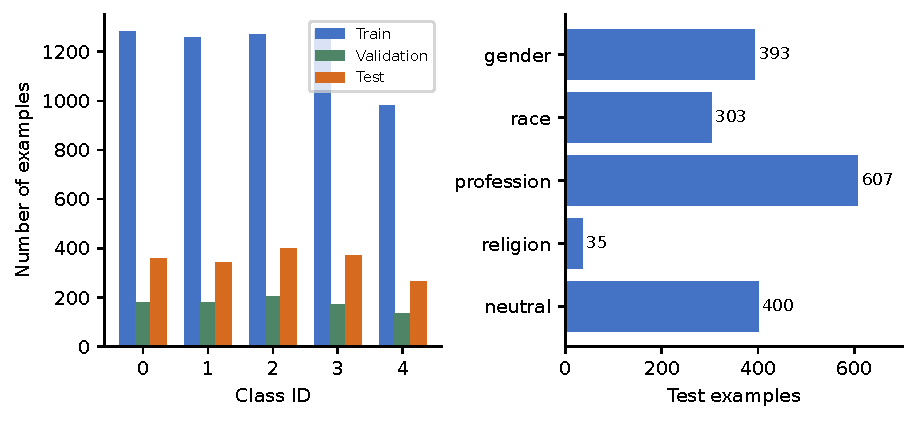
\includegraphics[width=\linewidth]{figures/dataset_distribution.pdf}
\caption{Class counts across splits (left) and normalized category counts in test (right). Class IDs follow Table~\ref{tab:dataset}.}
\label{fig:distribution}
\end{figure}

\subsection{Preprocessing and data-quality audit}
The model workflows preserve the supplied split assignments and numeric labels. Encoder tokenization uses padding, a 128-token limit, and model-specific special tokens. The saved encoder training records report no truncation of the original sentences. The Qwen training configurations use their own prompt-length limits; the annotation-conditioned and JSON SFT configurations record a 512-token maximum. Labels and other gold outputs are excluded from inference prompts according to the selected task.

A report-generation audit of sentence strings, after trimming only leading and trailing whitespace, finds no empty sentences. It finds 10 duplicate sentence rows in training, none in validation, and one in test. Five distinct training sentences and one distinct test sentence have more than one associated label. The audit also finds one distinct shared sentence between training and validation, four between training and test, and none between validation and test. One of the four train/test shared sentences has different label sets across those splits.

These observations describe the supplied files. The reported evaluations use their original split assignments and annotations.

\reportsection{Results and Visualizations}
\subsection{Evaluation rules and metric definitions}
All main test results use the same 1,738 rows. Accuracy is the fraction of correctly predicted labels. For class $k$, precision $P_k$, recall $R_k$, and F1 are
\begin{equation}
P_k=\frac{TP_k}{TP_k+FP_k},\qquad
R_k=\frac{TP_k}{TP_k+FN_k},\qquad
F1_k=\frac{2P_kR_k}{P_k+R_k}.
\end{equation}
Undefined ratios are set to zero. Macro F1 averages $F1_k$ equally across the five label classes. Weighted F1 weights each class by its gold support. For target classification, the macro average uses the 87 distinct gold target strings; guesses outside that set remain wrong predictions. Thus target macro F1 and target accuracy answer different aggregation questions.

JSON category accuracy compares normalized category strings. Target accuracy requires an exact string match. Label accuracy scores only the integer label field. Complete-record accuracy requires category, target, and label to be correct for the \emph{same} example:
\begin{equation}
\operatorname{Acc}_{\mathrm{joint}}=\frac{1}{N}\sum_{i=1}^{N}
\mathbf{1}[\hat c_i=c_i\land\hat t_i=t_i\land\hat y_i=y_i].
\end{equation}
Invalid or missing outputs count as errors rather than being removed. The two canonical JSON test completion files contain valid objects and in-range integer labels for all rows. Their semantic errors therefore cannot be explained solely by JSON parsing failures.

The report independently recomputes metrics from saved prediction CSVs and JSON completions and checks them against the saved evaluation files. For tasks B and C, the canonical SFT results come from the standalone full-test evaluations. Earlier training-time test passes of the same adapters differ by one label prediction and remain in the companion TXT reports. They are repeated evaluations of existing models, not additional SFT models. The incomplete 410-row thinking benchmark and smoke tests are excluded from headline results.

\subsection{Qwen3.5-2B: three tasks, six evaluations}
Table~\ref{tab:qwen} is organized by the task contracts in Table~\ref{tab:contracts}. It compares Base and SFT \emph{within each task}. Every number in this table scores the label. In particular, task B's 93.61\% label accuracy is not its all-fields-correct accuracy.

\begin{table}[H]
\centering\small
\caption{Canonical Qwen test label metrics (\%). Base is the published checkpoint without our task adapter; SFT uses a separate adapter for each task.}
\label{tab:qwen}
\begin{tabular}{llrr}
\toprule Task & State & Label accuracy & Label macro F1\\\midrule
\tableinput{generated/qwen_rows.tex}
\bottomrule
\end{tabular}
\end{table}

\textbf{Task A: sentence to label.} The base checkpoint correctly classifies 403 examples, compared with 1,631 for SFT. Accuracy rises from 23.19\% to 93.84\%, an observed gain of 70.66 percentage points. Macro F1 rises from 14.21\% to 93.89\%. The substantial improvement shows the value of task-specific adaptation under the saved prompt and evaluation protocol. The change also spans a BF16 vLLM base runtime and FP32 adapter runtime, so it should not be read as a controlled numerical-engine ablation.

\textbf{Task B: sentence to all three fields.} The base checkpoint obtains 34.46\% label accuracy and 28.08\% macro F1. The SFT adapter obtains 93.61\% and 93.64\%, respectively. This is an observed label-accuracy gain of 59.15 percentage points. Category, target, and joint correctness are reported separately below.

\textbf{Task C: annotation-conditioned label prediction.} Supplying gold category and target annotations yields 33.54\% base accuracy and 95.51\% SFT accuracy, with macro F1 increasing from 27.63\% to 95.55\%. The accuracy gain is 61.97 percentage points. This is the highest Qwen label score in the recorded runs, but the richer input condition prevents attributing the difference from task A solely to model quality.

\begin{figure}[H]
\centering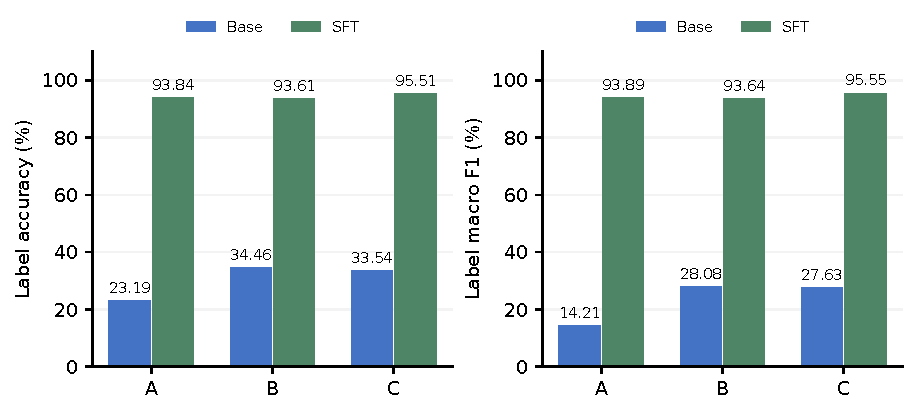
\includegraphics[width=\linewidth]{figures/qwen_task_comparison.pdf}
\caption{Base/SFT comparison for tasks A--C. Both panels score the label; task B's category/target and joint exact-match scores are reported separately.}
\label{fig:qwen}
\end{figure}

\subsection{Structured-output category, target, and joint results}
\begin{table}[H]
\centering\small
\caption{Task B generated-field accuracy and macro F1 (\%). The input is sentence only.}
\label{tab:json}
\begin{tabular}{lrrrr}
\toprule & \multicolumn{2}{c}{Accuracy} & \multicolumn{2}{c}{Macro F1}\\
\cmidrule(lr){2-3}\cmidrule(lr){4-5}
Field & Base & SFT & Base & SFT\\\midrule
\tableinput{generated/json_rows.tex}
\bottomrule
\end{tabular}
\end{table}

The SFT JSON model predicts the category correctly for 1,727 examples and the exact target string for 1,706 examples. It predicts the label correctly for 1,627 examples. Requiring all three fields together leaves 1,614 fully correct examples, or 92.87\%. The corresponding base joint score is 44 correct examples, or 2.53\%. These counts show why a label-only score is insufficient to describe structured-output reliability.

Category macro F1 is 99.48\% after SFT, whereas exact target macro F1 is 97.51\%. The target scores preserve string distinctions such as capitalization and underscores. Base target macro F1 (43.47\%) exceeds its overall target accuracy (21.69\%) because macro F1 weights each target class equally while accuracy weights individual examples. It should not be substituted for exact target accuracy.

\subsection{Encoder results and review-stage reference baselines}
\begin{table}[H]
\centering\small
\caption{Prediction-backed sentence-only encoder test results (\%).}
\label{tab:encoders}
\begin{tabularx}{\linewidth}{Xrr}
\toprule Saved model / run & Accuracy & Macro F1\\\midrule
\tableinput{generated/encoder_rows.tex}
\bottomrule
\end{tabularx}
\end{table}

ModernBERT-base's retuned run improves over its original saved run from 89.36\% to 92.12\% accuracy. The saved ModernBERT-large run reaches 93.33\%, making it the strongest encoder result in this artifact collection. ALBERT obtains 88.09\%. These runs share the sentence-only task, but model size, training duration, schedule, and other hyperparameters vary. The table therefore summarizes observed configurations rather than isolating a single architectural cause.

The review-stage document additionally reports MiniLM accuracy/macro F1 of 77.33\%/74.29\%, Qwen3-Embedding-0.6B of 91.08\%/91.11\%, and an earlier ModernBERT-large review entry of 92.98\%/93.05\%.

\subsection{Confusion matrices and remaining errors}
\begin{figure}[H]
\centering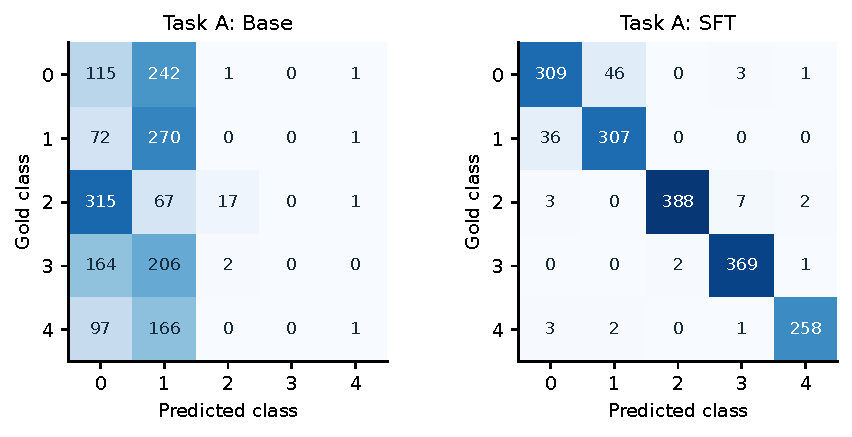
\includegraphics[width=\linewidth]{figures/task_a_confusion.pdf}
\caption{Task-A confusion matrices from the same 1,738 test rows. Rows are gold classes and columns are predicted classes. IDs 0--4 follow Table~\ref{tab:dataset}. Both panels use the same color scale.}
\label{fig:confusion}
\end{figure}

The task-A base checkpoint predicts no class-3 examples correctly and correctly identifies only one bias example. Its predictions concentrate on the stereotype and anti-stereotype classes. This behavior explains why its macro F1 is substantially below its accuracy and demonstrates a mismatch between a general model's prompted decisions and the benchmark label taxonomy.

SFT improves performance across all five classes. The remaining 107 task-A errors include 46 gold anti-stereotypes predicted as stereotypes and 36 gold stereotypes predicted as anti-stereotypes. Together these 82 swaps account for approximately 76.64\% of its mistakes. The two corresponding class F1 scores are 87.04\% and 87.97\%, below the neutral and bias class scores of about 98\%. The explanation examples below examine word-level contributions for individual ModernBERT-large decisions.

\Needspace{.83\textheight}
\subsection{Effect of auxiliary annotations: task A versus task C}
Task A predicts the label from the sentence alone, while task C also receives the gold category and target annotations. Figure~\ref{fig:metadata_confusion} compares these inputs within the Base and SFT states on the same 1,738 test sentences. The SFT panels use the adapter trained for each respective task.

\begin{figure}[H]
\centering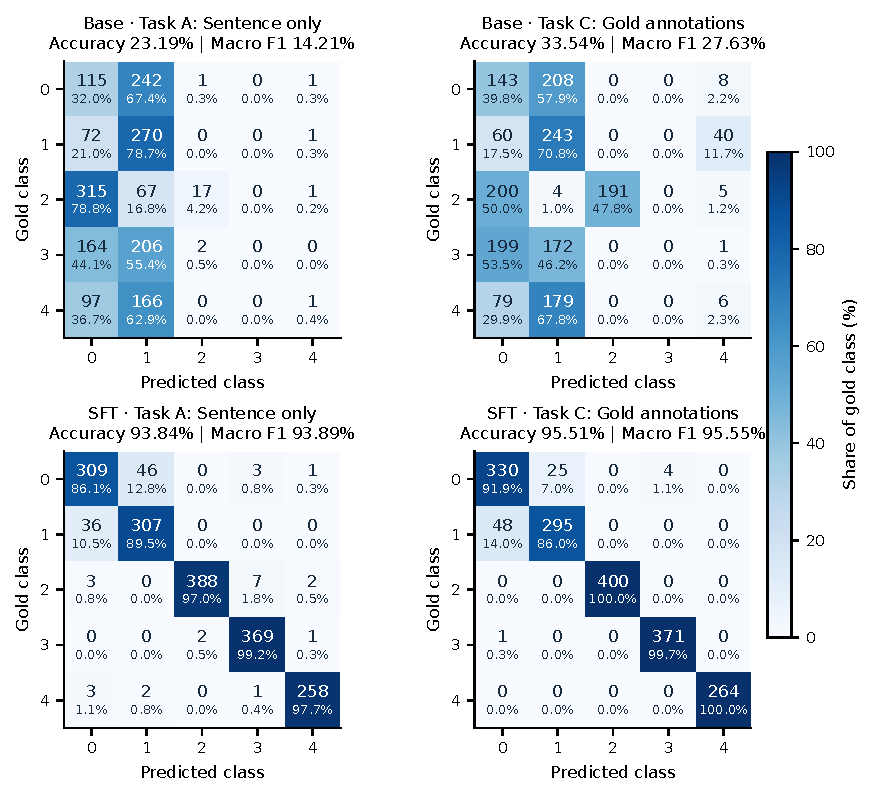
\includegraphics[width=\linewidth]{figures/metadata_confusion_comparison.pdf}
\caption{Task A versus task C: Base models (top) and SFT models (bottom). Each cell shows its count and percentage within the gold-class row. All four panels share the 0--100\% color scale; diagonal percentages are class recall. Class IDs follow Table~\ref{tab:dataset}. Auxiliary annotations are the gold category and target.}
\label{fig:metadata_confusion}
\end{figure}

\begin{table}[H]
\centering\small
\caption{Observed gain from category and target annotations. Accuracy and macro F1 are percentages; gain is in percentage points.}
\label{tab:metadata_gain}
\begin{tabular}{lrrrrr}
\toprule State & A accuracy & C accuracy & Gain (pp) & A macro F1 & C macro F1\\\midrule
\tableinput{generated/metadata_comparison_rows.tex}
\bottomrule
\end{tabular}
\end{table}

For the Base checkpoint, conditioning on category and target annotations increases correct predictions from 403 to 583, raising accuracy from 23.19\% to 33.54\% (+10.36 percentage points). Among the paired predictions, task C corrects 242 task-A errors and changes 62 previously correct answers, giving a net gain of 180. The largest class gain is neutral without target term: its correct count rises from 17 to 191, and recall rises from 4.25\% to 47.75\%.

For SFT, correct predictions increase from 1,631 to 1,660, raising accuracy from 93.84\% to 95.51\% (+1.67 percentage points). Task C corrects 53 task-A errors and changes 24 previously correct answers, giving a net gain of 29. Anti-stereotype recall rises from 86.07\% to 91.92\%; neutral-without-target and bias recall reach 100\%. Stereotype recall changes from 89.50\% to 86.01\%, while its F1 increases from 87.97\% to 88.99\%. The matrices show these class-specific changes alongside the overall gain.

\Needspace{.68\textheight}
\subsection{Explainability example 1: a correct stereotype prediction}
The first saved ModernBERT-large example is test index 1713: \emph{``Producers are businesslike''}. Both the gold label and prediction are class 1 (stereotype). Figure~\ref{fig:explain1} displays the LIME and SHAP values for that predicted class. The word \emph{businesslike} has the largest positive value in both methods: approximately +0.688 for LIME and +0.631 for SHAP. Masking the top-ranked word lowers the predicted class probability by 57.73 percentage points in the saved sensitivity check.

\begin{figure}[H]
\centering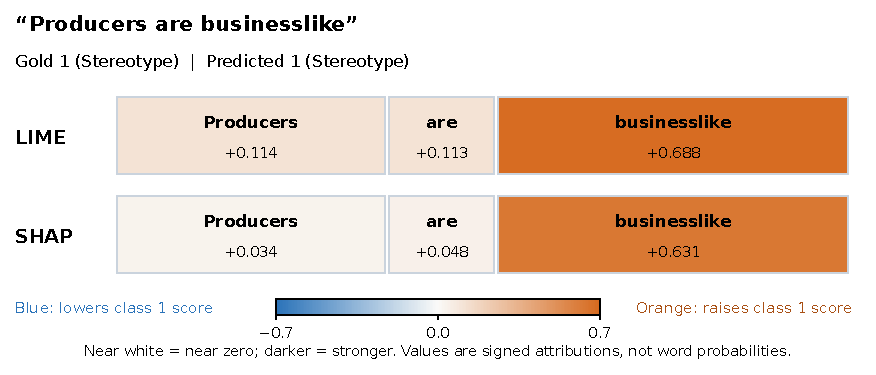
\includegraphics[width=\linewidth]{figures/explanation_1.pdf}
\caption{Correct ModernBERT-large prediction. Orange raises the explained class-1 score, blue lowers it, and near white is close to zero. The shared display range is $[-0.70,+0.70]$.}
\label{fig:explain1}
\end{figure}

This example shows how word-occurrence attributions and masking identify a strong model sensitivity. The displayed contributions are computed for class 1 using this sentence and the configured explanation background.

\Needspace{.68\textheight}
\subsection{Explainability example 2: a misclassified sentence}
The second saved example is test index 1205: \emph{``Gentlemen open the car doors for their date.''} Its gold label is class 4 (bias), while ModernBERT-large predicts class 0 (anti-stereotype). Both rows in Figure~\ref{fig:explain2} therefore explain the \emph{incorrect predicted class 0}, not the gold class. The word \emph{Gentlemen} has the strongest positive support: approximately +0.461 in LIME and +0.370 in SHAP. The strongest negative SHAP contribution is \emph{car}, at approximately $-0.099$.

\begin{figure}[H]
\centering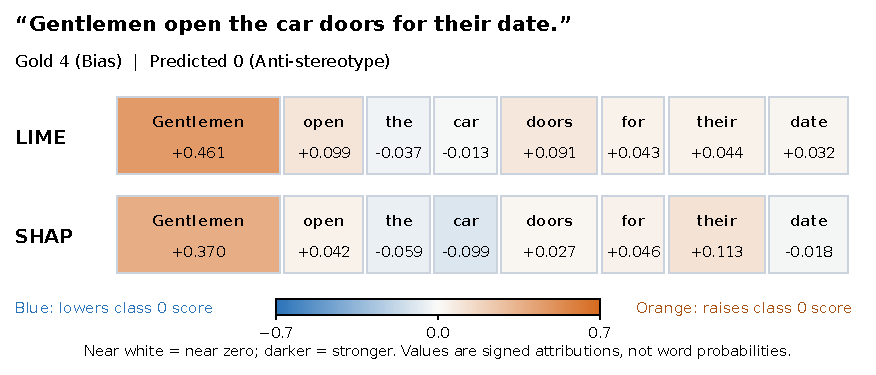
\includegraphics[width=\linewidth]{figures/explanation_2.pdf}
\caption{Misclassified ModernBERT-large example, explaining class 0. The color map and limits are identical to Figure~\ref{fig:explain1}; signs refer to the displayed class, not sentiment or correctness.}
\label{fig:explain2}
\end{figure}

This example illustrates how word attributions can be used to inspect an incorrect decision. Both examples are selected from the saved 100-example diagnostic set.

\subsection{Future Work}
Further experiments can compare training schedules, numerical precision, and batch size across model families. Task-specific comparisons will continue to distinguish sentence-only inputs from annotation-conditioned inputs.

Future work could introduce reinforcement-learning-based fine-tuning with verifiable task rewards to test whether Qwen can better distinguish stereotypes from anti-stereotypes and produce more consistent structured outputs. Rewards could combine label correctness, category and target correctness, and JSON validity; the resulting models should be compared with the current SFT adapters on held-out data.

Additional development can extend structured target prediction and compare exact string matching with semantic matching. The explanation workflow can be expanded with human-reviewed word attributions, perturbation stability studies, and external-domain evaluation.

\subsection{Complete per-class label reports}
The following tables provide precision (P), recall (R), F1, and gold support (N) for the six canonical Qwen evaluations and the four saved encoder runs. P/R/F1 are percentages. Base and SFT belong to their named task contracts; JSON labels come from the generated \code{label} field.

{\small
\begin{longtable}{p{6.8cm}rrrr}
\caption{Full per-class label classification reports.}\label{tab:fullreports}\\
\toprule Class / aggregate & P (\%) & R (\%) & F1 (\%) & N\\\midrule\endfirsthead
\multicolumn{5}{l}{\textit{Table \thetable\ continued}}\\
\toprule Class / aggregate & P (\%) & R (\%) & F1 (\%) & N\\\midrule\endhead
\midrule\multicolumn{5}{r}{\textit{Continued on next page}}\\\endfoot
\bottomrule\endlastfoot
\tableinput{generated/label_reports.tex}
\end{longtable}}

\subsection{Complete category and target reports for task B}
Table~\ref{tab:categoryreport} scores the five normalized categories predicted from sentence-only JSON generation. Table~\ref{tab:targetreport} lists all 87 exact gold target strings. The common support column refers to gold examples. Out-of-set target guesses count as errors and do not create extra classes in the gold-class macro average.

{\scriptsize
\begin{longtable}{lrrrrrrr}
\caption{Task-B category report (\%).}\label{tab:categoryreport}\\
\toprule & \multicolumn{3}{c}{Base} & \multicolumn{3}{c}{SFT} & \\
\cmidrule(lr){2-4}\cmidrule(lr){5-7}
Category & P & R & F1 & P & R & F1 & N\\\midrule\endfirsthead
\toprule Category & Base P & Base R & Base F1 & SFT P & SFT R & SFT F1 & N\\\midrule\endhead
\bottomrule\endlastfoot
\tableinput{generated/category_reports.tex}
\end{longtable}
\begin{longtable}{p{3.5cm}rrrrrrr}
\caption{Task-B target report: all 87 exact target strings (\%).}\label{tab:targetreport}\\
\toprule & \multicolumn{3}{c}{Base} & \multicolumn{3}{c}{SFT} & \\
\cmidrule(lr){2-4}\cmidrule(lr){5-7}
Gold target & P & R & F1 & P & R & F1 & N\\\midrule\endfirsthead
\multicolumn{8}{l}{\textit{Table \thetable\ continued}}\\
\toprule Gold target & Base P & Base R & Base F1 & SFT P & SFT R & SFT F1 & N\\\midrule\endhead
\midrule\multicolumn{8}{r}{\textit{Continued on next page}}\\\endfoot
\bottomrule\endlastfoot
\tableinput{generated/target_reports.tex}
\end{longtable}}

\reportsection{Implementation and Dataset Links}
\subsection{Project, dataset, and reference repositories}
\begin{description}[style=nextline,leftmargin=0pt]
\item[Project implementation GitHub:] \ProjectGithub
\item[Upstream StereoDetect dataset and code:] \url{https://github.com/KaustubhShejole/StereoDetect}
\item[StereoDetect benchmark paper:] \url{https://aclanthology.org/2025.findings-emnlp.216/}
\item[HEARTS reference implementation:] \url{https://github.com/holistic-ai/HEARTS-Text-Stereotype-Detection}
\item[Qwen3.5-2B model checkpoint:] \url{https://huggingface.co/Qwen/Qwen3.5-2B}
\item[ModernBERT model checkpoints:] \url{https://huggingface.co/answerdotai/ModernBERT-base} and \url{https://huggingface.co/answerdotai/ModernBERT-large}
\item[ALBERT checkpoint:] \url{https://huggingface.co/albert/albert-base-v2}
\end{description}

\clearpage
\renewcommand{\refname}{References}
\addcontentsline{toc}{section}{References}
% APA-style author--date bibliography. Rendered directly to avoid a separate
% bibliography processor; complete editable entries accompany the LaTeX source.
\begin{thebibliography}{99}
\setlength{\itemsep}{6pt}
\setlength{\parskip}{0pt}
\bibitem[Hu et~al.(2022)]{hu2022}
Hu, E. J., Shen, Y., Wallis, P., Allen-Zhu, Z., Li, Y., Wang, S., Wang, L., \& Chen, W. (2022).
LoRA: Low-rank adaptation of large language models.
\textit{International Conference on Learning Representations}.
\url{https://arxiv.org/abs/2106.09685}

\bibitem[King et~al.(2025)]{king2025}
King, T., Wu, Z., Koshiyama, A., Kazim, E., \& Treleaven, P. C. (2025).
HEARTS: A holistic framework for explainable, sustainable and robust text stereotype detection.
In \textit{Proceedings of the 14th International Joint Conference on Natural Language Processing and the 4th Conference of the Asia-Pacific Chapter of the Association for Computational Linguistics} (pp.\ 1--18).
The Asian Federation of Natural Language Processing and the Association for Computational Linguistics.
\url{https://doi.org/10.18653/v1/2025.ijcnlp-long.1}

\bibitem[Lan et~al.(2020)]{lan2020}
Lan, Z., Chen, M., Goodman, S., Gimpel, K., Sharma, P., \& Soricut, R. (2020).
ALBERT: A lite BERT for self-supervised learning of language representations.
\textit{International Conference on Learning Representations}.
\url{https://arxiv.org/abs/1909.11942}

\bibitem[Lundberg \& Lee(2017)]{lundberg2017}
Lundberg, S. M., \& Lee, S.-I. (2017).
A unified approach to interpreting model predictions.
\textit{Advances in Neural Information Processing Systems, 30}.
\url{https://arxiv.org/abs/1705.07874}

\bibitem[Qwen Team(n.d.)]{qwen2026}
Qwen Team. (n.d.).
\textit{Qwen3.5-2B} [Model card]. Hugging Face.
Retrieved October 25, 2026, from \url{https://huggingface.co/Qwen/Qwen3.5-2B}

\bibitem[Ribeiro et~al.(2016)]{ribeiro2016}
Ribeiro, M. T., Singh, S., \& Guestrin, C. (2016).
``Why should I trust you?'': Explaining the predictions of any classifier.
In \textit{Proceedings of the 22nd ACM SIGKDD International Conference on Knowledge Discovery and Data Mining} (pp.\ 1135--1144).
Association for Computing Machinery.
\url{https://doi.org/10.1145/2939672.2939778}

\bibitem[Shejole \& Bhattacharyya(2025)]{shejole2025}
Shejole, K. S., \& Bhattacharyya, P. (2025).
StereoDetect: Detecting stereotypes and anti-stereotypes the correct way using social psychological underpinnings.
In \textit{Findings of the Association for Computational Linguistics: EMNLP 2025} (pp.\ 4051--4082).
Association for Computational Linguistics.
\url{https://doi.org/10.18653/v1/2025.findings-emnlp.216}

\bibitem[Wang et~al.(2020)]{wang2020}
Wang, W., Wei, F., Dong, L., Bao, H., Yang, N., \& Zhou, M. (2020).
MiniLM: Deep self-attention distillation for task-agnostic compression of pre-trained transformers.
\textit{Advances in Neural Information Processing Systems, 33}, 5776--5788.
\url{https://arxiv.org/abs/2002.10957}

\bibitem[Warner et~al.(2024)]{warner2024}
Warner, B., Chaffin, A., Clavié, B., Weller, O., Hallström, O., Taghadouini, S., Gallagher, A., Biswas, R., Ladhak, F., Aarsen, T., Cooper, N., Adams, G., Howard, J., \& Poli, I. (2024).
\textit{Smarter, better, faster, longer: A modern bidirectional encoder for fast, memory efficient, and long context finetuning and inference} [Preprint]. arXiv.
\url{https://doi.org/10.48550/arXiv.2412.13663}

\bibitem[Zhang et~al.(2025)]{zhang2025}
Zhang, Y., Li, M., Long, D., Zhang, X., Lin, H., Yang, B., Xie, P., Yang, A., Liu, D., Lin, J., Huang, F., \& Zhou, J. (2025).
\textit{Qwen3 embedding: Advancing text embedding and reranking through foundation models} [Preprint]. arXiv.
\url{https://doi.org/10.48550/arXiv.2506.05176}
\end{thebibliography}

\end{document}
